\chapter{Bmad\_Standard Transfer Map Calculations}
\label{c:bmad.std}

For tracking and transfer map calculations (here generically called
``tracking''), \bmad has various methods that can be applied to a
given element (\sref{c:methods}). This chapter discusses the
\vn{bmad_standard} calculation that is the default for almost all
element types.

%-----------------------------------------------------------------
\section{Tracking with Non-Zero Offsets, Pitches, or Tilt}
\label{s:misalign.track}

\index{element reference coordinates}
The general procedure for tracking through an element makes use of
three sets of coordinates called \vn{``element reference
coordinates''} (or simply \vn{element coordinates}).  With
misalignments, the \vn{element coordinates} will stay fixed relative
to the element and will therefore shift with the element in the
laboratory frame of reference.  Here \vn{``misalignment''} is {\em
defined} to be any offset, pitch or tilt (\sref{s:offset}).

The three coordinate systems are named \vn{element entrance
coordinates}, \vn{element body coordinates}, and \vn{element exit
coordinates}. Without any \vn{``misalignments''}, the \vn{element
entrance coordinates} and \vn{element exit coordinates} are the same
as the laboratory coordinate system (\sref{s:ref}) at the entrance and
exit ends of the element respectively. [The one exception is when
a \vn{crystal} element has a non-zero \vn{psi_angle} value. See
\sref{s:crystal.ref}.] The \vn{body coordinate system} will be
discussed below. The general procedure for tracking a particle through
a given element is then a three step process: At the start, the
particle is at the entrance end of the element and the particle's
coordinates are given with respect to the laboratory coordinates.
\begin{enumerate}
\item
Transform from the laboratory reference coordinates to the element
entrance coordinates.
\item
Track through the element ignoring any misalignments ending up with
the particle at the exit end of the element with the particle's
coordinates given with respect to the element exit coordinates.
\item
Transform from the element exit coordinates to the laboratory
coordinates.
\end{enumerate}

\begin{figure}[tb]
  \centering
  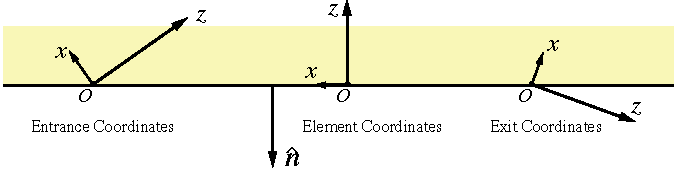
\includegraphics[width=5in]{photon-ele-coords.pdf}
  \caption[Crystal and Mirror Element Coordinates.]
{Element coordinates for \vn{crystal} and \vn{mirror} elements. For
clarity, the three coordinate systems are displaced from each
other. In actuality, the origin $\Bf O$ of all three is the same.
$\bfhat n$ is the normal to the element surface}
  \label{f:photon.ele.coords}
\end{figure}

\index{crystal}\index{mirror}
For \vn{straight} elements (\sref{s:ref}), all three element
coordinate systems are the same and, in this case, all three are
simply referred to as \vn{element coordinates}.  For \vn{crystal}
(\sref{s:crystal}) and \vn{mirror} (\sref{s:mirror}) elements, the
non-straight reference trajectory complicates the geometry. For these
elements, the three element coordinate systems are shown in
Fig.~\ref{f:photon.ele.coords}. In the \vn{element entrance
coordinates}, the surface normal $\bfhat n$ is in the $x$-$z$ plane
and the $y$ axis will be parallel to the surface. This is a
consequence of the convention that, with no tilt, the bend is about
the $y$-axis (\sref{s:global}). The \vn{element body coordinates} are
derived from the \vn{element entrance coordinates} by a rotation about
the $y$-axis so that in the body coordinates, the $x$ axis points
opposite the $\bfhat n$ vector and the $z$-axis is parallel to the
surface. The \vn{element exit coordinates} will generally have it's
$y$-axis aligned with the $y$-axes of the other two coordinate
systems. The exceptional case occurs for a \vn{crystal} element when
\vn{phi_angle} is nonzero (\sref{s:crystal.ref}).

%-----------------------------------------------------------------
\section{Transformation for Straight Elements Between 
Laboratory and Element Coordinates}
\label{s:straight-lab-ele}

It is assumed that pitches are are small so that second
order terms can be ignored.

%-----------------------------------------------------------------
\subsection{Transformation from Laboratory to Element Coordinates}

The transformation from the laboratory coordinates to
element coordinates for an element that has a
straight reference trajectory through it is accomplished in a number of steps.
\begin{enumerate}
\item
Track as in a drift a distance \vn{s_offset_tot}.
\item
Apply offsets and pitches
\begin{align}
  x_1    &= x_0 - x_{off} + \frac{L}{2} x'_{pitch} \CRNO
  p_{x1} &= p_{x0} - (1 + p_{z0}) \, x'_{pitch} \CRNO
  y_1    &= y_0 - y_{off} + \frac{L}{2} y'_{pitch} \\
  p_{y1} &= p_{x0} - (1 + p_{z0}) \, y'_{pitch} \CRNO
  z_1    &= z_0 + x'_{pitch} \, x_1 + y'_{pitch} \, y_1 - 
    \frac{L}{4} (x^{\prime2}_{pitch} + y^{\prime2}_{pitch}) \nonumber
\end{align}
Notice that $z_1$ is written in terms of $x_1$ and $y_1$
\item
Apply any tilt $\theta_t$
\begin{align}
  x_2    &=  x_1    \, \cos\theta_t + y_1    \, \sin\theta_t \CRNO
  p_{x2} &=  p_{x1} \, \cos\theta_t + p_{y1} \, \sin\theta_t \CRNO
  y_2    &= -x_1    \, \sin\theta_t + y_1    \, \cos\theta_t \\
  p_{y2} &= -p_{x1} \, \sin\theta_t + p_{y1} \, \cos\theta_t \nonumber
\end{align}
\end{enumerate}

%-----------------------------------------------------------------
\subsection{Transformation from Element to Laboratory Coordinates}

The back transformation from element to laboratory coordinates is
accomplished by the transformation
\begin{enumerate}
\item
Apply any tilt $\theta_t$
\begin{align}
  x_1    &=  x_0    \, \cos\theta_t - y_0    \, \sin\theta_t \CRNO
  p_{x1} &=  p_{x0} \, \cos\theta_t - p_{y0} \, \sin\theta_t \CRNO
  y_1    &=  x_0    \, \sin\theta_t + y_0    \, \cos\theta_t \\
  p_{y1} &=  p_{x0} \, \sin\theta_t + p_{y0} \, \cos\theta_t \nonumber
\end{align}
\item
Apply offsets and pitches
\begin{align}
  x_2    &= x_1 + x_{off} + \frac{L}{2} x'_{pitch}     \CRNO
  p_{x2} &= p_{x1} + (1 + p_{z1}) \, x'_{pitch}        \CRNO
  y_2    &= y_1 + y_{off} + \frac{L}{2} y'_{pitch}     \\
  p_{y2} &= p_{x1} + (1 + p_{z1}) \, y'_{pitch}        \CRNO
  z_2    &= z_1 + x'_{pitch} \, x_1 + y'_{pitch} \, y_1 - 
    \frac{L}{4} (x^{\prime2}_{pitch} + y^{\prime2}_{pitch})      \nonumber
\end{align}
\item
Track as in a drift a distance \vn{-s_offset_tot}.
\end{enumerate}


%-----------------------------------------------------------------
\section[Mirror and Crystal Elements]{Transformation for Mirror and Crystal Elements Between 
Laboratory and Element Coordinates}
\label{s:photon-lab-ele}

\index{mirror}\index{crystal}
It is assumed that pitches are are small so that second
order terms can be ignored.

%-----------------------------------------------------------------
\subsection{Transformation from Laboratory to Element Coordinates}

\index{s_offset_tot}
With photons, the intensities must also be transformed.
The transformation from the the entrance laboratory coordinates to
the entrance element coordinates is:
\begin{enumerate}
\item
Track as in a drift a distance \vn{s_offset_tot}.
\item
\index{x_offset}\index{x_pitch}\index{y_offset}\index{y_pitch}
Apply offsets and pitches: The effective ``length'' of the element is
zero (\sref{s:mirror.coords}) so the origin of the element coordinates
is the same point around which the element is pitched so
\begin{align}
  x_1    &= x_0 - x_{off} \CRNO
  p_{x1} &= p_{x0} - (1 + p_{z0}) \, x'_{pitch} \CRNO
  y_1    &= y_0 - y_{off} \\
  p_{y1} &= p_{x0} - (1 + p_{z0}) \, y'_{pitch} \CRNO
  z_1    &= z_0 + x'_{pitch} \, x_1 + y'_{pitch} \, y_1 \nonumber
\end{align}
where $x_{off} \equiv \vn{x_offset}$, $x'_{pitch} \equiv \vn{x_pitch}$, etc.
\item
Apply \vn{tilt} and \vn{tilt_err}:
\begin{align}
  \begin{pmatrix} x_2 \\ y_2 \end{pmatrix} &=
    \bR (\theta_{tot}) \,   
  \begin{pmatrix} x_1 \\ y_1 \end{pmatrix} \CRNO
  \begin{pmatrix} p_{x2} \\ p_{y2} \end{pmatrix} &=
    \bR (\theta_{tot}) \, 
  \begin{pmatrix} p_{x1} \\ p_{y1} \end{pmatrix} \label{xyrtxy} \\ 
  \begin{pmatrix} \bE_{x2} \\ \bE_{y2} \end{pmatrix} &=
    \bR (\theta_{tot}) \,   \begin{pmatrix} \bE_{x1} \\ \bE_{y1} \end{pmatrix} \nonumber
\end{align}
where $\bE$ is shorthand notation for
\Begineq
  \bE \equiv E \, e^{i \, \phi}
\Endeq
with $E$ being the field intensity and $\phi$ being the field phase angle.
In the above equations $\bR$ is the rotation matrix
\Begineq
  \bR(\theta) = \begin{pmatrix} \cos\theta & \sin\theta \\ -\sin\theta & \cos\theta \end{pmatrix}
\Endeq
\index{tilt}\index{tilt_err}\index{tilt_corr}
with $\theta_{tot}$ being 
\Begineq
  \theta_{tot}  = 
  \begin{cases}
    \vn{tilt} + \vn{tilt_err} + \vn{tilt_corr} & \vn{for crystal elements} \\
    \vn{tilt} + \vn{tilt_err} & \vn{for mirror elements}
  \end{cases}
\Endeq
The \vn{tilt_corr} correction is explained below.
\item
\index{graze_angle_err}
Apply \vn{graze_angle_err} ($\theta_{gerr}$):
\begin{align}
  p_{x3} &= p_{x2} + \theta_{gerr} \CRNO
  z_3    &= z_2 - x_2 \, \theta_{gerr} 
\end{align}
\end{enumerate}

%-----------------------------------------------------------------
\subsection{Transformation from Element to Laboratory Coordinates}

The back transformation from exit element coordinates to exit
laboratory coordinates is accomplished by the transformation
  \begin{enumerate}
  \item
Apply \vn{graze_angle_err}:
\begin{align}
  p_{x1} &= p_{x0} - \theta_{gerr} \CRNO
  z_1    &= z_0 + x_0 \, \theta_{gerr} 
\end{align}
  \item
Apply \vn{tilt} and \vn{tilt_err}: \vn{tilt} rotates the exit
laboratory coordinates with respect to the exit element coordinates in
the same way \vn{tilt} rotates the entrance laboratory coordinates
with respect to the entrance element coordinates. The forward and back
transformations are thus just inverses of each other.  With
\vn{tilt_err}, this is not true. \vn{tilt_err}, unlike \vn{tilt}, does
not rotate the output laboratory coordinates.  There is the further
complication in that \vn{tilt_err} is a rotation about the {\em
entrance} laboratory coordinates. The first step is to express
\vn{tilt_err} with respect to the exit coordinates. This is done with
the help of the $\bS$ matrix of \Eq{r00ls} with $\alpha$ given by
\Eq{agg}. The effect of the \vn{tilt_err} can be modeled as a rotation
vector $\Bf e_{in}$ in the entrance laboratory coordinates pointing
along the $z$-axis
\Begineq
 \Bf e_{in} = (0, 0, \mbox{tilt_err})
\Endeq
In the exit laboratory coordinates, the vector $\Bf e_{out}$ is
\Begineq
  \Bf e_{out} = \bS \, \Bf e_{in}
\Endeq
The $z$ component of $\Bf e_{out}$ combines with \vn{tilt} to give
the transformation
\begin{align}
  \begin{pmatrix} x_2 \\ y_2 \end{pmatrix} &=
    \bR (-\theta_{t}) \,   \begin{pmatrix} x_1 \\ y_1 \end{pmatrix} \CRNO
  \begin{pmatrix} p_{x2} \\ p_{y2} \end{pmatrix} &=
    \bR (-\theta_{t}) \,   \begin{pmatrix} p_{x1} \\ p_{y1} \end{pmatrix} \\
  \begin{pmatrix} \bE_{x2} \\ \bE_{y2} \end{pmatrix} &=
    \bR (-\theta_{t}) \,   \begin{pmatrix} \bE_{x1} \\ \bE_{y1} \end{pmatrix} \nonumber
\end{align}
where $\theta_t$ is $\mbox{tilt} + \Bf e_{out,z}$. The $x$ and $y$ components
of $\Bf e_{out}$ give rotations around the $x$ and $y$ axes
\begin{align}
  p_{x3} &= p_{x2} - \Bf e_{out,y} \CRNO
  p_{y3} &= p_{y2} + \Bf e_{out,x} \\
  z_3    &= z_2 + x_2 \, \Bf e_{out,y} - y_2 \, \Bf e_{out,x}
\end{align}
  \item
Apply pitches: Since pitches are defined with
respect to the entrance laboratory coordinates, they have to be
translated to the exit laboratory coordinates
\Begineq
  \bP_{out} = \bS \, \bP_{in}
\Endeq
where $\bP_{in} = (x'_{pitch}, y'_{pitch}, 0)$ is the pitch vector in
the entrance laboratory frame and $\bP_{out}$ is the vector in the exit
laboratory frame. The transformation is then
\begin{align}
  p_{x4} &= p_{x3} - \bP_{out,y} \CRNO
  p_{y4} &= p_{y3} + \bP_{out,x} \\
  z_4    &= z_3 + x_3 \, \bP_{out,y} - y_3 \, \bP_{out,x}
\end{align}
  \item
Apply offsets: Again, offsets are defined with respect to the
entrance laboratory coordinates. Like pitches, the translation is
\Begineq
  \bO_{out} = \bS \, \bO_{in}
\Endeq
where $\bO_{in} = (x_{off}, y_{off}, s_{off})$ is the offset in the
entrance laboratory frame. The transformation is
\begin{align}
  x_5 &= x_4 + \bO_{out,x} - p_{x4} \, \bO_{out,z} \CRNO
  y_5 &= y_4 + \bO_{out,y} - p_{y4} \, \bO_{out,z} \\
  z_5 &= z_4 + \bO_{out,z} 
\end{align}
  \end{enumerate}

%-----------------------

\begin{figure}[tb]
  \centering
  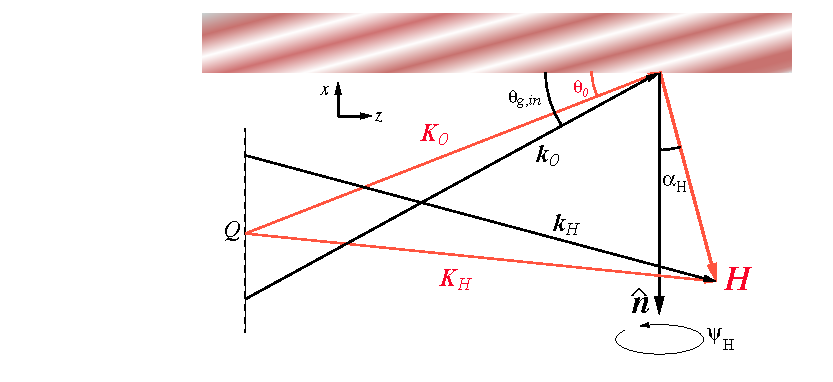
\includegraphics[width=5in]{crystal-diffraction.pdf}
  \caption[Crystal diffraction diagram.]
{Reciprocal space diagram showing crystal diffraction for Bragg
reflection. The coordinates shown are the element body 
coordinates. All points in the diagram are in the plane of the paper
except for the tip of $\bH$.  $\bK_{0}$ and $\Bf K_{H}$ are the wave
vectors inside the crystal and $\Bf k_{0}$ and $\Bf k_{H}$ are the
wave vectors outside the crystal. The reference photon traveling along
the reference trajectory has $\bK_0$ and $\bK_H$ originating at the
$Q$ point.}
  \label{f:crystal.diffraction}
\end{figure}

%-----------------------------------------------------------------
\section{Crystal Element Tracking}
\label{s:crystal.tracking}

\textit{\large [Crystal tracking developed by Jing Yee Chee, Ken Finkelstein, and David Sagan]}

%-----------------------------------------------------------------
\subsection{Crystal Element Reference Trajectory}
\label{s:crystal.ref}

Crystal diffraction is modeled using dynamical diffraction theory. The
notation here follows Batterman and Cole\cite{b:batterman}. Before any
photon tracking is done, the incoming grazing angle $\theta_{g,in}$
and outgoing grazing angle $\theta_{g,out}$ must be computed to orient
the reference trajectory with respect to the crystal surface.
Fig.~\ref{f:crystal.diffraction} shows the geometry of the
problem. The graze angles are calculated such that a photon with the
reference energy on the reference trajectory will be in the center of
the Darwin curve. That is, the internal wave vectors $\bK_0$ and
$\bK_H$ originate from the $Q$ point (See \cite{b:batterman} Figs.~8
and 29).

The calculation of the incoming graze angle $\theta_{g,in}$
(\vn{graze_angle_in}) is as follows. The external incoming wave vector
$\Bf k_0$, which is coincident with the element entrance trajectory,
lies along the element entrance coordinates $z$ axis. In element body
coordinates (which will be the coordinate system used henceforth),
$\Bf k_0$ thus lies in the $x$-$z$ plane. $\bK_0$ is related to $\Bf
k_0$ via Batterman Eq.~(25)
\Begineq
  \bK_0 = \Bf k_0 + q_a \, \bfhat n
\Endeq
where the value of $q_a$ is determined, in part, by the requirement on
the lengths of the vectors
\begin{align}
  |\bf k_0| &= |\bf k_H| = \frac{1}{\lambda} 
  \label{kk1l1} \\
  |\bK_0| &= |\bK_H| = \frac{1}{\lambda \, (1 + \delta)}
  \label{kk1l2}
\end{align}
where 
\Begineq
  \delta = \frac{\lambda^2 r_e}{2 \, \pi \, V} \, |F_0|
\Endeq
with $r_e$ begin the classical electron radius, $V$ the unit cell
volume, and $F_0$ is the $F_{(0,0,0)}$ structure factor. Since both
$\bf k_0$ and $\bfhat n$ lie in the $x$-$z$ plane, $\bK_0$ lies in the
$x$-$z$ plane and can thus be written in the form
\Begineq
  \bK_0 = \frac{1}{\lambda \, (1 + \delta)} \, 
    \begin{pmatrix}
    \sin\theta_0 \\
    0 \\
    \cos\theta_0
    \end{pmatrix}
  \label{k1l1d}
\Endeq
where $\theta_0$ is the angle between $\bK_0$ and $z$ as shown in
Fig.~\ref{f:crystal.diffraction}.
The vectors $\bK_0$ and $\bH$ must add up to the reciprocal lattice vector $\bK_H$
\Begineq
  \bK_H + \bK_0 + \bH
\Endeq
Using
\Begineq
  \bH = \frac{1}{d}
  \begin{pmatrix} -\cos \alpha_H \\ \sin \alpha_H \, \sin \psi_H \\ \sin \alpha_H \, \cos \psi_H \end{pmatrix}
  \label{h1daa}
\Endeq
gives
\Begineq
  \frac{1}{\lambda \, (1 + \delta)} \, \bfhat K_H
  =
  \frac{1}{\lambda \, (1 + \delta)} \, 
  \begin{pmatrix} \sin\theta_0 \\ 0 \\ \cos\theta_0 \end{pmatrix}
  +
  \frac{1}{d}
  \begin{pmatrix} -\cos \alpha_H \\ \sin \alpha_H \, \sin \psi_H \\ \sin \alpha_H \, \cos \psi_H \end{pmatrix}
  \label{1l1dk}
\Endeq
where $\bfhat K_H$ has unit length and $\alpha_H$ (\vn{alpha_angle})
and $\psi_H$ (\vn{psi_angle}) characterize the orientation of $H$.
Taking the length of both sides gives
\Begineq
  \frac{\lambda (1 + \delta)}{2 \, d} = \cos\alpha_H \, \sin\theta_0 = 
  \sin\alpha_H \, \cos\psi_H \, \cos\theta_0
\Endeq
Solving for $\theta_0$ gives
\Begineq
  \theta_0 = \sin^{-1} \frac{\lambda (1 + \delta)}{2 \, d \, \sqrt{1 - \sin^2\alpha_H \, \sin^2\psi_H}} +
  \tan^{-1} (\tan\alpha_H \, \cos\psi_H)
\Endeq
From this, the incoming graze angle is
\Begineq
  \cos\theta_{g,in} = \frac{\cos\theta_0}{1 + \delta}
\Endeq

The outgoing reference wave vector $k_H$ is computed by noting that
vectors $\bK_H$ and $\Bf k_h$ share the same $y$ and $z$ coordinates. Thus,
from \Eq{1l1dk} 
\begin{align}
  k_{H,y} &= \frac{1}{d} \sin\alpha_H \, \sin\psi_H \CRNO
  k_{H,z} &= \frac{1}{d} \sin\alpha_H \, cos\psi_H + \frac{1}{\lambda \, (1 + \delta)} \, \cos\theta_0
  \label{k1dap}
\end{align}
And the $x$ component is obtained from \Eq{kk1l1}
\Begineq
  k_{H,x} = -\sqrt{\frac{1}{\lambda^2} - k_{H,y}^2 - k_{H,z}^2}
  \label{k1lkk}
\Endeq
The total bending angle of the reference trajectory is then
\Begineq
  \theta_{bend} = \tan^{-1} \left( \frac{ | \Bf k_0 \times \Bf k_H | }{\Bf k_0 \cdot \Bf k_H} \right)
\Endeq
The outgoing graze angle $\theta_{g,out}$ is then {\em defined} to be
the difference between the total bend angle and the entrance graze angle.
\Begineq
  \theta_{g,out} \equiv \theta_{bend} - \theta_{g,in}
\Endeq

In order to track photons, the transformations between coordinate
systems are needed. In particular, as shown below, a ``tilt
correction'' needs to be applied when $\psi_H$ is nonzero.  Since the
tilt correction is independent of any misalignments, it is assumed
here that there are no misalignments. The full transformations between
coordinate systems with misalignments are given in section
\sref{s:photon-lab-ele}

Without misalignments, and with
$\psi_H$ zero, the transformation matrix $T_{in}$ between laboratory
entrance coordinates and element entrance coordinates is (as it is for
every other type of element) just the unit matrix. That is, the two
coordinate systems are identical. Furthermore, the transformation $M_{in}$ from
element entrance coordinates to body coordinates is a rotation around
the $y$ axis
\Begineq
  M_{in} = \begin{pmatrix}
     \cos\theta_{g,in} & 0 & \sin\theta_{g,in} \\
     0                 & 1 & 0                 \\
    -\sin\theta_{g,in} & 0 & \cos\theta_{g,in} \\
  \end{pmatrix}
  \label{mt0t010}
\Endeq
The transformation from element body coordinates to element exit
coordinates is another rotation around the $y$ axis with angle
$\theta_{g,out}$ and the transformation from element exit coordinates
to laboratory exit coordinates is the unity matrix. Thus, the combined
transformation from laboratory entrance to laboratory exit coordinates
is a rotation around the $y$ axis of $\theta_{g,in}+\theta_{g,out}$ as
explained in section \sref{s:global}.

\index{tilt}\index{psi_angle}
When $\psi_H$ is non-zero the situation is complicated since, if the
above transformations for the coordinate systems are used, the vector
$\Bf k_H$ would be bent out of the $x$-$z$ plane.  By {\em
definition}, the reference trajectory has the form given by \Eq{lrca1}
with the $\bT$ matrix depending only upon the \vn{tilt} parameter.  To
satisfy \Eq{lrca1}, the crystal must be reorientated to keep the $\Bf
k_H$ vector in the $x$-$z$ plane of the laboratory entrance
coordinates.  The reorientation is done by rotating the crystal about
the laboratory entrance $\Bf z$ axis by an amount $\theta_{corr}$
(\vn{tilt_corr}). With this ``tilt correction'' rotation, the
transformation $\bT_{in}$ between laboratory entrance coordinates and
element entrance coordinates is
\Begineq
  \bT_{in} = 
  \begin{pmatrix}
    \cos\theta_{corr} & -\sin\theta_{corr} & 0 \\
    \sin\theta_{corr} &  \cos\theta_{corr} & 0 \\
    0                 &  0                 & 1                
  \end{pmatrix}
\Endeq
The transformation from element entrance coordinates to element body
coordinates is not affected by a finite $\psi_H$ and so \Eq{mt0t010}
is unmodified. The $\Bf k_H$ vector, expressed in laboratory entrance
coordinates, is $\bT_{in}^{-1} \, \bM_{in}^{-1} \, \Bf k_H$ where the
components of $\Bf k_H$ are given by \Eqs{k1dap} and \eq{k1lkk}. To
satisfy \Eq{lrca1}, this vector must have zero $y$ component
\Begineq
  \left( \bT_{in}^{-1} \, \bM_{in}^{-1} \, \Bf k_H \right) \cdot
  \begin{pmatrix} 0 \\ 1 \\ 0 \end{pmatrix}
  = 0
\Endeq
Solving gives
\Begineq
  \theta_{corr} = \tan^{-1} 
  \frac{k_{H,y}}{k_{H,z} \, \sin\theta_{g,in} - k_{H,x} \, \cos\theta_{g,in}}
\Endeq
The transformation $\bM_{out}$ from element body coordinates to
element exit coordinates is now obtained by requiring that the total
transformation from laboratory entrance to laboratory exit coordinates
be the $\bftilde S$ matrix given in \Eq{lrca1}
\Begineq
  \bM_{out} \, \bM_{in} \, \bT_{in} = 
  \begin{pmatrix}
    \cos\theta_{bend} & 0 & -\sin\theta_{bend} \\
    0          & 1 & 0           \\
    \sin\theta_{bend} & 0 & \cos\theta_{bend}
  \end{pmatrix}
\Endeq
In the above equation, the transformation $T_{out}$ from element exit
coordinates to laboratory exit coordinates has been dropped since it
is the unit matrix independent of $\psi_H$.

%-----------------------------------------------------------------
\subsection{Crystal Element Tracking}

The starting photon coordinates are specified in the laboratory
entrance coordinates. The transformation from laboratory entrance
coordinates to element entrance coordinates $\bftilde k_0$ is given in
\sref{s:photon-lab-ele}. The transformation to element body
coordinates $k_{in}$ is
\begin{equation}
  \Bf k_0 =  \bM_{in} \, \bftilde k_0
\end{equation}
with $\bM_{in}$ given by \Eq{mt0t010}.
The outgoing wave vector $k_H$ is related to $k_0$ via
\Begineq
  \Bf k_H =  \Bf k_0 + \bH + q_t \, \bfhat n
\Endeq
where $q_t$ is determined by using \Eqs{k1l1d} and \eq{h1daa} in \Eq{kk1l1}
\Begineq
  \frac{1}{\lambda} =
  \left| \frac{1}{d}
  \begin{pmatrix} -\cos \alpha_H \\ \sin \alpha_H \, \sin \psi_H \\ \sin \alpha_H \, \cos \psi_H \end{pmatrix}
  +
  \frac{1}{\lambda \, (1 + \delta)} \, 
  \begin{pmatrix} \sin\theta_0 \\ 0 \\ \cos\theta_0 \end{pmatrix}
  -
  \begin{pmatrix} q_t \\ 0 \\ 0 \end{pmatrix} \right|
\Endeq  

To compute the field amplitude of the outgoing photon, the equation to
be solved is (\cite{b:batterman} Eq.~(21))
\Begineq
  \xi_0 \, \xi_H = \frac{1}{4} \, k^2 \, P^2 \, \Lambda^2 \, F_H \, F_{\bar H}
\Endeq
where $\xi_0$ and $\xi_H$ are given by \cite{b:batterman} Eq.~(18)
and $P$ is the polarization factor
\Begineq
  P = 
  \begin{cases}
    1               & \sigma \mbox{ polarization state} \\
    \cos 2\theta_g  & \pi \mbox{ polarization state}
  \end{cases}
\Endeq
$2\theta_g$ is the angle between $\bK_0$ and $\bK_H$ which is well
approximated by $\theta_{g,in} + \theta_{g,out}$.

The solution is (\cite{b:batterman} Eq.~(31))
\begin{align}
  \xi_0 &= \frac{1}{2} \, k \, |P| \, \Gamma \, [F_H \, F_{\bar H}]^{1/2} \, 
    |b|^{1/2} \, [\eta \pm (\eta^2 + \sign(b))^{1/2}] \CRNO
  \xi_H &= \frac{1}{2} \, k \, |P| \, \Gamma \, [F_H \, F_{\bar H}]^{1/2} \, 
    \frac{1}{|b|^{1/2} \, [\eta \pm (\eta^2 + \sign(b))^{1/2}]}
\end{align}
where $\sign$ is the sign function
\Begineq
  \sign(b) \equiv \begin{cases} 1 & b > 0 \\ -1 & b < 0 \end{cases}
\Endeq
and $\eta$ is given by \cite{b:blasdell} Eq.~(5)
\Begineq
  \eta = \frac{-b \, a + \Gamma \, F_0 \, (1 - b)}{2 \, \Gamma \, |P| \, \sqrt{|b| \, F_H \, F_{\bar H}}}
\Endeq
with the asymmetry factor $b$ for the photon being tracked being given
by \cite{b:blasdell} Eq.~(3)
\Begineq
  b \equiv \frac{\bfhat n \cdot \bfhat k_0}{\bfhat n \cdot \widehat{{\Bf k_0 + \bH}}}
\Endeq
and the angular deviation variable $a$ is given by \cite{b:blasdell} Eq.~(4)
\Begineq
  a \equiv \frac{H^2 + 2 \, \Bf k_0 \cdot \bH}{k_0^2}
\Endeq

%-----------------------------------------------------------------
\section{Hamiltonian for a Magnetic Element}
\label{s:mag.hamiltonian}

Without any electric fields, the Hamiltonian is
\Begineq
  H = p_z - (1 + g \, x) \sqrt{(1 + p_z)^2 - (p_x - a_x)^2 - (p_y - a_y)^2} - 
  (1 + g \, x) \, a_s
  \label{h1gx1}
\Endeq
Here $(x, p_x, y, p_y, z, p_z)$ are the canonical coordinates
(\sref{s:phase.space}), $g = 1/\rho$ with $\rho$ being the local
radius of curvature of the reference particle, and $\Bf a(x,y,s)$ is
the normalized vector potential which is related to the vector
potential $\Bf A(x,y,s)$ via
\Begineq
  \Bf a = \frac{q \, \Bf A}{P_0 \, c}
\Endeq
The equations of motion are
\begin{align}
  \frac{dq_i}{ds} &= \frac{\partial H}{\partial p_i} \CRNO
  \frac{dp_i}{ds} &= -\frac{\partial H}{\partial q_i}
  \label{rshp}
\end{align}

Assuming mid--plane symmetry of the magnetic field, so
that $a_x$ and $a_y$ can be set to zero\cite{b:madphysics}, The vector
potential up to second order is (cf.~\Eq{byx0b})
\Begineq
  a_s = -k_0 \left( x - \frac{g \, x^2}{2 (1 + g\, x)} \right) -
  \frac{1}{2} k_1 \left( x^2 - y^2 \right)
\Endeq

\label{paraxial approximation}
Using the paraxial approximation (\sref{s:phase.space}), \Eq{h1gx1} becomes
\Begineq
  H = \frac{(p_x - a_x)^2}{2 (1 + p_z)} + \frac{(p_y - a_y)^2}{2 (1 + p_z)} - 
  (1 + g \, x) \, a_s 
  \label{hpapa}
\Endeq

Once the transverse trajectory has been calculated, the longitudinal position
$z_2$ at the exit end of an element is obtained from symplectic
integration of \Eq{hpapa}
\Begineq
  z_2 = z_1 - \frac{1}{2 (1 + p_{z1})^2} \int \! ds \, 
  \left[ (p_x - a_x)^2 + (p_y - a_y)^2 \right] - \int \! ds \, g \, x
  \label{zz121p}
\Endeq
where $z_1$ is the longitudinal position at the entrance end of the element.
Using the equations of motion \Eqs{rshp} this can also be rewritten as
\Begineq
  z_2 = z_1 - \frac{1}{2} \int \! ds \, 
  \left[ \left( \frac{dx}{ds} \right)^2 + \left( \frac{dy}{ds} \right)^2 \right] - 
  \int \! ds \, g \, x
  \label{zz12sx}
\Endeq

For some elements, \vn{bmad_standard} uses a truncated Taylor map for
tracking.  For elements without electric fields where the particle
energy is a constant, the transfer map for a given coordinate $r_i$
may be expanded in a Taylor series
\Begineq
  r_{i,2} \rightarrow m_i + \sum_{j = 1}^4 m_{ij} \, r_{j,1} + 
  \sum_{j = 1}^4 \sum_{k = j}^4 m_{ijk} \, r_{j,1} \, r_{k,1} + \ldots
\Endeq
where the map coefficients $m_{ij\cdots}$ are functions of $p_z$.  For
linear elements, the transfer map is linear for the transverse
coordinates and quadratic for $r_i = z$.

%-----------------------------------------
\section{BeamBeam Element Tracking}
\label{s:beambeam.std}
\index{beambeam}

A beam-beam element (\sref{s:bbi}) simulates the effect on a tracked
particle of an opposing beam of particles moving in the opposite
direction. The opposing beam, called the ``strong'' beam, is assumed
to be Gaussian in shape.

The strong beam is divided up into \vn{n_slice} equal charge (not
equal thickness) slices. Propagation through the strong beam involves
a kick at the charge center of each slice with drifts in between the
kicks. The kicks are calculated using the standard Bassetti--Erskine
complex error function formula\cite{b:talman}.  Even though the strong
beam can have a finite \vn{sig_z} the length of the element is always
considered to be zero. This is achieved by adding drifts at either end
of any tracking so that the longitudinal starting point and ending
point are identical. The longitudinal $s$--position of the
\vn{BeamBeam} element is at the center of the strong bunch. For
example, with \vn{n_slice} = 2 the calculation would proceed as
follows:
\begin{enumerate}
  \item  Start with the reference particle at the center of the strong bunch.
  \item  Propagate (drift) backwards to the center of the first slice.
  \item  Apply the beam--beam kick due to the first slice.
  \item  Propagate (drift) forwards to the center of the second slice.
  \item  Apply the beam--beam kick due to the second slice.
  \item  Propagate (drift) backwards to end up with the reference particle
     at the center of the strong bunch.
\end{enumerate}

%-----------------------------------------
\section{Bend Element: Fringe Tracking}
\label{s:.bend.fringe.std}
\index{sbend}

The transformation for the entrance face of an \vn{sbend} is
\begin{align}
  p_{x2} &= p_{x1} + k_x \, x_1 \CRNO
  p_{y2} &= p_{y1} + k_y \, y_1
\end{align}
where
\begin{align}
  k_x &= g_{tot} \, \tan(e_1) \CRNO
  k_y &= -g_{tot} \, \tan \left[ e_1 - 2 \, |g_{tot}| \, f_{int} \,  h_{gap} \, 
    \frac{1 + \sin(e1)^2}{\cos(e_1)} \right]
\end{align}
where $g_{tot}$ is the total bending strength (design +
error). Similar equations are used for tracking the exit edge of the
bend.

%-----------------------------------------
\section{Bend Element: Body Tracking}
\label{s:bend.body.std}
\index{sbend}

The Hamiltonian for the body of an \vn{sbend} is
\Begineq
  H = (k_0 - g) x - g \, x \, p_z + 
  \frac{1}{2}\left( (k_1 + g \, k_0) x^2 - k_1 \, y^2 \right) +
  \frac{p_x^2 + p_y^2}{2 (1 + p_z)} 
\Endeq

This is simply solved
\begin{align}
  x_2    &= c_x \, (x - x_c) + s_x \, \frac{p_{x1}}{1 + p_{z1}} + x_c \CRNO
  p_{x2} &= \tau_x \, \om_x^2 \, \, (1 + p_{z1}) \, s_x \, (x -x_c) + c_x \, p_{x1} \CRNO
  y_2    &= c_y \, y_1 + s_y \, \frac{p_{y1}}{1 + p_{z1}} \CRNO
  p_{y2} &= \tau_y \, \om_y^2 \, \, (1 + p_{z1}) \, s_y \, y_1 + c_y \, p_{y1} \\
  z_2    &= z_1 + m_5 + m_{51} (x - x_c) + m_{52} p_{x1} + m_{511} \, (x-x_c)^2 \, + \CRNO
         &\hspace*{20ex} m_{512} \, (x-x_c) \, p_{x1} + m_{522} \, p_{x1}^2 + 
                         m_{533} \, y^2 + m_{534} \, y_1 \, p_{y1} + m_{544} \, p_{y1}^2 \CRNO
  p_{z2} &= p_{z1} \nonumber
\end{align}
where 
\begin{alignat}{2}
  k_x &= k_1 + g \, k_0 & \qqquad
  \om_x &\equiv \sqrt{\frac{|k_x|}{1 + p_{z1}}} \CRNO
  x_c &= \frac{g \, (1 + p_{z1}) - k_0}{k_x} & \qqquad
  \om_y &\equiv \sqrt{\frac{|k_1|}{1 + p_{z1}}} 
\end{alignat}
and
\begin{alignat}{6}
         &\hspace*{3ex}  && k_x > 0          &\hspace*{3ex}& k_x < 0 & \qqquad
         &\hspace*{3ex}  && k_1 > 0          &\hspace*{3ex}& k_1 < 0 \CRNO
     c_x &=   && \cos  (\om_x \, L)               && \cosh (\om_x \, L) & \qqquad
     c_y &=   && \cosh (\om_y \, L)               && \cos  (\om_y \, L) \CRNO
     s_x &=   && \frac{\sin  (\om_x \, L)}{\om_x} && \frac{\sinh (\om_x \, L)}{\om_x} & \qqquad
     s_y &=   && \frac{\sinh (\om_y \, L)}{\om_y} && \frac{\sin  (\om_y \, L)}{\om_y} \\
  \tau_x &=   && {-}1             && {+}1             & \qqquad
  \tau_y &=   && {+}1             && {-}1             \nonumber
\end{alignat}
and
\begin{alignat}{2}
  m_5     &= -g \, x_c \, L & \qqquad & \CRNO
  m_{51}  &= -g \, s_x & \qqquad
  m_{52}  &= \frac{\tau_x \, g}{1 + p_{z1}} \, \frac{1 - c_x}{\om_x^2} \CRNO
  m_{511} &= \frac{\tau_x \,\, \om_x^2}{4} \, (L - c_x \, s_x) & \qqquad
  m_{533} &= \frac{\tau_y \,\, \om_y^2}{4} \, (L - c_y \, s_y) \CRNO
  m_{512} &= \frac{-\tau_x \,\, \om_x^2}{2 \, (1 + p_{z1})} \, s_x^2 & \qqquad
  m_{534} &= \frac{-\tau_y \,\, \om_y^2}{2 \, (1 + p_{z1})} \, s_y^2 \CRNO
  m_{522} &= \frac{-1}{4 \, (1 + p_{z1})^2} \, (L + c_x \, s_x) & \qqquad
  m_{544} &= \frac{-1}{4 \, (1 + p_{z1})^2} \, (L + c_y \, s_y) \nonumber
\end{alignat}

%-----------------------------------------
\section{Drift Element Tracking}
\label{s:drift.std}
\index{drift} 

\Eq{h1gx1} for a drift has $\Bf a = 0$ and $g = 0$. The Hamiltonian for a
drift is then
\Begineq
  H = \frac{p_x^2 + p_y^2}{2 (1 + p_z)} 
\Endeq
This gives the map
\begin{align}
  x_2    &= x_1 + \frac{L \, p_{x1}}{1 + p_{z1}} \CRNO
  p_{x2} &= p_{x1}  \CRNO
  y_2    &= y_1 + \frac{L \, p_{y1}}{1 + p_{z1}} \CRNO
  p_{y2} &= p_{y1}  \\
  z_2    &= z_1 - \frac{L \, (p_{x1}^2 + p_{y1}^2)}{2 (1 + p_{z1})^2} \CRNO
  p_{z2} &= p_{z1} \nonumber
\end{align}

%-----------------------------------------
\section{Kicker, Hkicker, Vkicker, and Elseparator Element Tracking}
\label{s:kicker.std}
\index{kicker}
\index{hkicker}
\index{vkicker}
\index{elseparator}

The Hamiltonian for a horizontally deflecting kicker or separator is
\Begineq
  H = \frac{p_x^2 + p_y^2}{2 (1 + p_z)} - k_0 \, x 
\Endeq
This gives the map
\begin{align}
  x_2    &= x_1 + \frac{1}{1 + p_{z1}} \, \left( L \, p_{x1} + \frac{1}{2} k_0 \, L^2 \right) \CRNO
  p_{x2} &= p_{x1} + k_0 \, L \CRNO
  y_2    &= y_1 + \frac{L \, p_{y1}}{1 + p_{z1}} \CRNO
  p_{y2} &= p_{y1}  \\
  z_2    &= z_1 - \frac{L}{2 (1 + p_{z1})^2} \, 
    \left( p_{x1}^2 + p_{y1}^2 + p_{x1} \, k_0 \, L + \frac{1}{3} k_0^2 \, L^2 \right) \CRNO
  p_{z2} &= p_{z1} \nonumber
\end{align}
The generalization when the kick is not in the horizontal plane is easily derived.

%-----------------------------------------
\section{Lcavity Element Tracking}
\label{s:lcavity.std}
\index{lcavity}

The transverse trajectory through an \vn{Lcavity} is modeled using equations
developed by Rosenzweig and Serafini\cite{b:rosenzweig} with
\Begineqs
  b_0 &= 1 \CRNO
  b_{-1} &= 1 
\Endeqs
and all other $b_n$ set to zero.

The transport through the body (R\&S Eq.~(9)) has been modified to give the 
correct phase-space area at non ultra-relativistic energies:
\Begineq
  \begin{pmatrix}
    x \\ 
    x'
  \end{pmatrix}_2 = 
  \begin{pmatrix}
    m_{11}                      & \beta_1 \, m_{12} \\
    \frac{1}{\beta_2} \, m_{21} & \frac{\beta_1}{\beta_2} \, m_{22} 
  \end{pmatrix}
  \,
  \begin{pmatrix}
    x \\ 
    x'
  \end{pmatrix}_1
\Endeq
where the $m_{ij}$ are the matrix elements from R\&S Eq.~(9) and the 
$\beta$ are the standard relativistic factors. With this, the determinate 
of the matrix is $\beta_1 \, \gamma_1 / \beta_2 \, \gamma_2$.

The change in $z$ going through a cavity is calculated by first calculating the particle
transit time $\Delta t$
\begin{align}
  c \, \Delta t &= \int_{s_1}^{s_2} \!\! ds \,\, \frac{1}{\beta(s)} \CRNO
  &= \int_{s_1}^{s_2} \!\! ds \, \frac{E}{\sqrt{E^2 - (mc^2)^2}} \\
  &= \frac{c \, P_{z2} - c \, P_{z1}}{G} \nonumber
\end{align}
where it has been assumed that the accelerating gradient $G$ is
constant through the cavity. In this equation $\beta = v / c$, $E$ is
the energy, and $P_{z1}$ and $P_{z2}$ are the entrance and exit
momenta. Using \Eq{zbctt}, the change in $z$ is thus
\Begineq
  z_2 = \frac{\beta_2}{\beta_1} \, z_1 - 
  \beta_2 \, 
  \left(
  \frac{c \, P_{z2} - c \, P_{z1}}{G} - 
  \frac{c \, \Pbar_{z2} - c \, \Pbar_{z1}}{\BAR G}
  \right)
\Endeq
where $\Pbar$ and $\BAR G$ are the momentum and gradient of the
reference particle.

The derivatives are straight forward if tedious
\begin{align}
  m_{55} &= \frac{dz_2}{dz_1} = 
    \frac{\beta_2}{\beta_1} + 
    \frac{z_2 \, m_{65}}{\beta_2} \frac{d\beta_2}{dp_{z2}} - 
    \frac{\beta_2}{G} \frac{dcP_2}{dz_1} +
    \frac{\beta_2 \, c \, (P_2 - P_1) \, c P_2}{L \, G^2 \, E_2} 
      \frac{dcP_2}{dz_1} \CRNO
  m_{56} &= \frac{dz_2}{dp_{z1}} = 
    \frac{-\beta_2 \, z_1}{\beta_1^2} \frac{d\beta_1}{dp_{z1}} + 
    \frac{z_2 \, m_{66}}{\beta_2} \frac{d\beta_2}{dp_{z2}} -
    \frac{\beta_2 ( c \Pbar_{2} \, m_{66} - c \Pbar_{1})}{G} \CRNO
  m_{65} &= \frac{dp_{z2}}{dz1} =
    \frac{E_2}{cP_2 \, c\Pbar_{2}} \frac{cP_1 \, c\Pbar_{1}}{E_1}  \\
  m_{66} &= \frac{dp_{z2}}{dp_{z1}} = 
    \frac{E_2}{cP_2} \frac{G \, L}{c \Pbar_{2}} \frac{2 \, \pi \, f \, \sin\phi}{c}
    \nonumber
\end{align}
where
\begin{align}
  \frac{d\beta_1}{dp_{z1}}  &= \frac{(mc^2)^2}{E_1^3} \, c\Pbar_{1} \CRNO
  \frac{d\beta_2}{dp_{z2}}  &= \frac{(mc^2)^2}{E_2^3} \, c\Pbar_{2} \\
  \frac{dcP_2}{dz_1}        &= m_{65} \, c\Pbar_{2}  \nonumber
\end{align}

%-----------------------------------------
\section{Mirror Element Tracking}
\label{s:mirror.std}
\index{mirror}

Tracking through

%-----------------------------------------
\section{Octupole Element Tracking}
\label{s:octupole.std}
\index{octupole}

The Hamiltonian for an upright octupole is
\Begineq
  H = \frac{p_x^2 + p_y^2}{2 (1 + p_z)} + \frac{k_3}{24} (x^4 - 6 \, x^2 \, y^2 + y^4)
\Endeq

An octupole is modeled using a kick-drift-kick model.

%-----------------------------------------
\section{Quadrupole Element Tracking}
\label{s:quadrupole.std}
\index{quadrupole}

The \vn{bmad_standard} calculates the transfer map through an upright
quadrupole and then transforms that map to the laboratory frame.

The Hamiltonian for an upright quadrupole is
\Begineq
  H = \frac{p_x^2 + p_y^2}{2 (1 + p_z)} + \frac{k_1}{2} (x^2 - y^2)
\Endeq
This is simply solved
\begin{align}
  x_2    &= c_x \, x_1 + s_x \, \frac{p_{x1}}{1 + p_{z1}} \CRNO
  p_{x2} &= \tau_x \, \om^2 \, \, (1 + p_{z1}) \, s_x \, x_1 + c_x \, p_{x1} \CRNO
  y_2    &= c_y \, y_1 + s_y \, \frac{p_{y1}}{1 + p_{z1}} \CRNO
  p_{y2} &= \tau_y \, \om^2 \, \, (1 + p_{z1}) \, s_y \, y_1 + c_y \, p_{y1} \\
  z_2    &= z_1 + m_{511} \, x_1^2 + m_{512} \, x_1 \, p_{x1} + m_{522} \, p_{x1}^2 + 
                   m_{533} \, y_1^2 + m_{534} \, y_1 \, p_{y1} + m_{544} \, p_{y1}^2 \CRNO
  p_{z2} &= p_{z1} \nonumber
\end{align}
where 
\Begineq
  \om \equiv \sqrt{\frac{|k_1|}{1 + p_{z1}}}
\Endeq
and
\begin{alignat}{6}
         &\hspace*{3ex}  && k_1 > 0          &\hspace*{3ex}& k_1 < 0 & \qqquad
         &\hspace*{3ex}  && k_1 > 0          &\hspace*{3ex}& k_1 < 0 \CRNO
     c_x &=   && \cos  (\om \, L) && \cosh (\om \, L) & \qqquad
     c_y &=   && \cosh (\om \, L) && \cos  (\om \, L) \CRNO
     s_x &=   && \frac{\sin  (\om \, L)}{\om} && \frac{\sinh (\om \, L)}{\om} & \qqquad
     s_y &=   && \frac{\sinh (\om \, L)}{\om} && \frac{\sin  (\om \, L)}{\om} \\
  \tau_x &=   && {-}1             && {+}1             & \qqquad
  \tau_y &=   && {+}1             && {-}1             \nonumber
\end{alignat}
with this
\begin{alignat}{2}
  m_{511} &= \frac{\tau_x \,\, \om^2}{4} \, (L - c_x \, s_x) & \qqquad
  m_{533} &= \frac{\tau_y \,\, \om^2}{4} \, (L - c_y \, s_y) \CRNO
  m_{512} &= \frac{-\tau_x \,\, \om^2}{2 \, (1 + p_{z1})} \, s_x^2 & \qqquad
  m_{534} &= \frac{-\tau_y \,\, \om^2}{2 \, (1 + p_{z1})} \, s_y^2 \\
  m_{522} &= \frac{-1}{4 \, (1 + p_{z1})^2} \, (L + c_x \, s_x) & \qqquad
  m_{544} &= \frac{-1}{4 \, (1 + p_{z1})^2} \, (L + c_y \, s_y) \nonumber
\end{alignat}


%-----------------------------------------
\section{RFcavity Element Tracking}
\label{s:rfcavity.std}
\index{rfcavity}

%-----------------------------------------
\section{Sextupole Element Tracking}
\label{s:sextupole.std}
\index{sextupole}

The Hamiltonian for an upright octupole is
\Begineq
  H = \frac{p_x^2 + p_y^2}{2 (1 + p_z)} + \frac{k_2}{6} (x^3 - 3 \, x \, y^2)
\Endeq

A sextupoles modeled using a kick-drift-kick model.

%-----------------------------------------
\section{Sol\_Quad Element Tracking}
\label{s:sol.quad.std}
\index{sol_quad}

The Hamiltonian is
\Begineq
  H = \frac{(p_x + \frac{k_s }{2}\, y)^2}{2 (1 + p_z)} + 
  \frac{(p_y - \frac{k_s}{2} \, x)^2}{2 (1 + p_z)} + \frac{k_1}{2} (x^2 - y^2)
\Endeq
Solving the equations of motion gives
\begin{align}
  x_2    &= m_{11} \, x_1 + m_{12} \, p_{x1} + m_{13} \, y_1 + m_{14} \, p_{y1} \CRNO
  p_{x2} &= m_{21} \, x_1 + m_{22} \, p_{x1} + m_{23} \, y_1 + m_{24} \, p_{y1} \CRNO
  y_2    &= m_{31} \, x_1 + m_{32} \, p_{x1} + m_{33} \, y_1 + m_{34} \, p_{y1} \CRNO
  p_{y2} &= m_{41} \, x_1 + m_{42} \, p_{x1} + m_{43} \, y_1 + m_{44} \, p_{y1} \\
  z_2    &= z_1 + \sum_{j = 1}^4 \sum_{k = j}^4 m_{5jk} \, r_j \, r_k  \CRNO
  p_{z2} &= p_{z1} \nonumber
\end{align}
where
\begin{alignat}{2}
  m_{11} &= \frac{1}{2 \, f} \, \left( f_{0+} \, c + f_{0-} \, c_h \right) & \qqquad
  m_{31} &= -m_{24} \CRNO
  m_{12} &= \frac{1}{2 \, f \, (1 + p_{z1})} \, 
            \left( \frac{f_{++}}{\om_+} \,  s + \frac{f_{--}}{\om_-} \, s_h \right) & \qqquad
  m_{32} &= -m_{14} \CRNO
  m_{13} &= \frac{\ks}{4 \, f} \, 
            \left( \frac{f_{+-}}{\om_+} \, s +\frac{f_{-+}}{\om_-} \, s_h \right) & \qqquad
  m_{33} &= \frac{1}{2 \, f} \, \left( f_{0-} \, c + f_{0+} \, c_h \right) \CRNO
  m_{14} &= \frac{\ks}{f \, (1 + p_{z1})} \, \left( -c + c_h \right) & \qqquad
  m_{34} &= \frac{1}{2 \, f \, (1 + p_{z1})} \, 
            \left( \frac{f_{+-}}{\om_+} \, s + \frac{f_{-+}}{\om_-} \, s_h \right) \CRNO
  m_{21} &= \frac{-(1 + p_{z1})}{8 \, f} \, 
            \left( \frac{\xi_{1+}}{\om_+} \, s + \frac{\xi_{2+}}{\om_-} s_h \right) & \qqquad
  m_{41} &= -m_{23} \\
  m_{22} &= m_{11} & \qqquad
  m_{42} &= -m_{13} \CRNO
  m_{23} &= \frac{\ks^3 \, (1 + p_{z1})}{4 \, f} \, \left( c - c_h \right) & \qqquad
  m_{43} &= \frac{-(1 + p_{z1})}{8 \, f} \, 
            \left( \frac{\xi_{1-}}{\om_+} \, s + \frac{\xi_{2-}}{\om_-} \, s_h \right) \CRNO
  m_{24} &= \frac{\ks}{4 \, f} \, 
            \left( \frac{f_{++}}{\om_+} \, s + \frac{f_{--}}{\om_-} \, s_h \right) & \qqquad
  m_{44} &= m_{33} \nonumber
\end{alignat}
and
\begin{alignat}{2}
  \kone        &= \frac{k_1}{1 + p_{z1}} & \qqquad 
  \ks          &= \frac{k_s}{1 + p_{z1}} \CRNO
  f            &= \sqrt{\ks^4 + 4 \, \kone^2} & \qqquad
  f_{\pm0}     &= f \pm \ks^2 \CRNO
  f_{0\pm}     &= f \pm 2 \, \kone & \qqquad
  f_{\pm\pm}   &= f \pm \ks^2 \pm 2 \, \kone \CRNO
  \om_+        &= \sqrt{\frac{f_{+0}}{2}} & \qqquad
  \om_-        &= \sqrt{\frac{f_{-0}}{2}} \\
  s            &= \sin (\om_+ \, L) & \qqquad
  s_h          &= \sinh (\om_- \, L) \CRNO
  c            &= \cos (\om_+ \, L) & \qqquad
  c_h          &= \cosh (\om_- \, L) \CRNO
  \xi_{1\pm} &= \ks^2 \, f_{+\mp} \pm 4 \, \kone \, f_{+\pm} & \qqquad
  \xi_{2\pm} &= \ks^2 \, f_{-\pm} \pm 4 \, \kone \, f_{-\mp} \nonumber
\end{alignat}

The $m_{5jk}$ terms are obtained via \Eq{zz121p}
\begin{align}
  m_{5jk} = - \frac{\tau_{jk}}{2 (1 + p_{z1})^2} \int \! ds \, 
  & \left[ 
    \left( m_{2j} + \frac{k_s}{2} \, m_{3j} \right) \, 
    \left( m_{2k} + \frac{k_s}{2} \, m_{3k} \right)   
  \right. + \\
  & \hspace*{15ex} \left.
    \left( m_{4j} - \frac{k_s}{2} \, m_{1j} \right) \, 
    \left( m_{4k} - \frac{k_s}{2} \, m_{1k} \right) 
  \right] \nonumber
\end{align}
where
\Begineq
  \tau_{jk} = 
  \begin{cases}
    1 & j = k \\
    2 & j \ne k 
  \end{cases}
\Endeq
The needed integrals involve the product of two trigonometric or
hyperbolic functions. These integrals are trivial to do but the
explicit equations for $m_{5jk}$ are quite long and in the interests of
brevity are not reproduced here.

%-----------------------------------------
\section{Solenoid Element Tracking}
\label{s:solenoid.std}
\index{solenoid}

The Hamiltonian is
\Begineq
  H = \frac{ \left( p_x + \frac{k_s}{2} \, y \right)^2}{2 \, (1 + p_z)} + 
  \frac{ \left( p_y - \frac{k_s}{2} \, x \right)^2}{2 \, (1 + p_z)} 
\Endeq
The solution is
\begin{align}
  x_2    &= \frac{1 + c}{2} \, x_1 + \frac{s}{k_s} \, p_{x1} +
           \frac{s}{2} \, y_1 + \frac{1 - c}{k_s} \, p_{y1} \CRNO
  p_{x2} &= \frac{-k_s \, s}{4} \, x_1 + \frac{1 + c}{2} \, p_{x1} - 
           \frac{k_s \, (1 - c)}{4} \, y_1 + \frac{s}{2} \, p_{y1} \CRNO
  y_2    &= \frac{-s}{2} \, x_1 - \frac{1 - c}{k_s} \, p_{x1} +
           \frac{1 + c}{2} \, y_1 + \frac{s}{k_s} \, p_{y1} \\      
  p_{y2} &= \frac{k_s \, (1 - c)}{4} \, x_1 + \frac{-s}{2} \, p_{x1} -
            \frac{k_s \, s}{4} \, y_1 + \frac{1 + c}{2} \, p_{y1} \CRNO 
  z_2    &= z_1 + \frac{L}{2 \, (1 + p_{z1})^2} \, 
                   \left[ \left( p_{x1} + \frac{k_s}{2} \, y_1 \right)^2 +
                          \left( p_{y1} - \frac{k_s}{2} \, x_1 \right)^2 \right] \CRNO
  p_{z2} &= p_{z1} \nonumber
\end{align}
where
\begin{align}
  c &= \cos \left( \frac{k_s}{2} \, L \right) \CRNO
  s &= \sin \left( \frac{k_s}{2} \, L \right)
\end{align}

%-----------------------------------------
\section{Map\_type Wiggler Element Tracking}
\label{s:wiggler.map.std}
\index{wiggler}

\index{wiggler}
As discussed in \sref{s:wiggler}, \bmad wiggler elements are
split into two classes: \vn{map type} and \vn{periodic type}. The 
\vn{map type} wigglers are modeled using the method of Sagan, Crittenden,
and Rubin\cite{b:wiggler}. In this model the magnetic field is written
as a sum of terms $B_i$
\Begineq
  \bfB(x,y,s) = \sum_i \bfB_i(x, y, s; C, k_x, k_y, k_s, \phi_s)
\Endeq 
Each term $B_i$ is specified using five numbers: 
$(C, k_x, k_y, k_s, \phi_s)$. A term can take one of three forms: The first
form is
\begin{alignat}{4}
  B_x &= -&C &\dfrac{k_x}{k_y} & \sin(\kxx) \sinh(\kyy) \cos(\ksss) \CRNEG
  B_y &=  &C &                 & \cos(\kxx) \cosh(\kyy) \cos(\ksss) \CRNEG
  B_s &= -&C &\dfrac{k_s}{k_y} & \cos(\kxx) \sinh(\kyy) \sin(\ksss) \label{f1} \\
  & \makebox[1pt][l]{with $k_y^2 = k_x^2 + k_s^2$ .} &&&  \nonumber
\end{alignat}
The second form is
\begin{alignat}{4}
  B_x &=  &C &\dfrac{k_x}{k_y} & \sinh(\kxx) \sinh(\kyy) \cos(\ksss) \CRNEG
  B_y &=  &C &                 & \cosh(\kxx) \cosh(\kyy) \cos(\ksss) \CRNEG
  B_s &= -&C &\dfrac{k_s}{k_y} & \cosh(\kxx) \sinh(\kyy) \sin(\ksss) \label{f2} \\
  & \makebox[1pt][l]{with $k_y^2 = k_s^2 - k_x^2$ ,} &&&  \nonumber
\end{alignat}
The third form is
\begin{alignat}{4}
  B_x &=  &C &\dfrac{k_x}{k_y} & \sinh(\kxx) \sin(\kyy) \cos(\ksss) \CRNEG
  B_y &=  &C &                 & \cosh(\kxx) \cos(\kyy) \cos(\ksss) \CRNEG
  B_s &= -&C &\dfrac{k_s}{k_y} & \cosh(\kxx) \sin(\kyy) \sin(\ksss) \label{f3} \\
  & \makebox[1pt][l]{with $k_y^2 = k_x^2 - k_s^2$ .} &&& \nonumber
\end{alignat}
The relationship between $k_x$, $k_y$, and $k_s$ ensures that
Maxwell's equations are satisfied.

There is no \vn{bmad_standard} tracking for a \vn{map_type}
\vn{wiggler}. The following describes the \vn{symp_lie_bmad} type tracking.
The Hamiltonian for the wiggler is 
\Begineq
  H = H_x + H_y + H_z
\Endeq
where
\begin{align}
  H_x &= \frac{p_x^2}{2 (1 + \delta)} \CRNO
  H_y &= \frac{(p_y - A_y)^2}{2 (1 + \delta)} \\
  H_s &= - A_s \nonumber
\end{align}
And the vector potential $\bfA$ is obtained from $\bfB$ via
\begin{align}
  A_x(x,y,s) &= 0 \CRNO
  A_y(x,y,s) &=  \int_0^x d\wt x \, B_z(\wt x, y, s) 
  \label{a0a0a0} \\
  A_s(x,y,s) &= -\int_0^x d\wt x \, B_y(\wt x, y, s) \nonumber
\end{align}

For tracking, the wiggler is broken up into a number of slices set by
the element's \vn{ds_step} attribute. For each slice, the tracking
uses a quadratic symplectic integrator $I$:
\Begineq
  I = T_{s/2} \; I_{x/2} \; I_{y/2} \; I_s \; I_{y/2} \; I_{x/2} \; T_{s/2}
\Endeq
$T_{s/2}$ is just a translation of the $s$ variable:
\Begineq
  s \rightarrow s + \frac{ds}{2}
\Endeq
And the other integrator components are
\begin{align}
  I_{x/2} &= \exp \left( : -\frac{ds}{2} H_x : \right) \CRNO
  I_{y/2} &= \exp \left( : -\frac{ds}{2} H_y : \right) \\
  I_{s}   &= \exp \left( : -ds \, H_s : \right) \nonumber
\end{align}
The evaluation if $I_{y/2}$ is tricky since it involves both transverse
position and momentum variables. The trick is to split the integration into three parts
\begin{align}
  I_{y/2} &= \exp \left( : -\frac{ds}{2} \frac{(p_y - A_y)^2}{2 (1 + \delta)} : \right) \CRNO
  &= \exp \left( : -\int A_y \, dy : \right) \,
     \exp \left( : -\frac{ds}{2} \frac{p_y^2}{2 (1 + \delta)} : \right) \,
     \exp \left( : \int A_y \, dy : \right)
  \label{ids2}
\end{align}
Given the form of the of the magnetic field of \Eqs{f1}, \eq{f2}, and
\eq{f3}, the integrals in \Eq{a0a0a0} and \eq{ids2} are easily calculated.

%-----------------------------------------
\section{Periodic\_Type Wiggler Element Tracking}
\label{s:wiggler.periodic.std}
\index{wiggler}

The horizontal motion looks like a drift with a superimposed
sinusoidal oscillation. It is assumed that there is an integer number
of periods in the oscillation so that the exit horizontal coordinates
can be calculated from the initial coordinates using the equations for
a drift. The vertical motion is a quadratic superimposed with a
octupole. Vertical motion is calculated using a kick-drift-kick model.

\vn{Periodic type} wigglers use a simplified model where the magnetic
field components are
\begin{alignat}{1}
  B_y &= \hphantom{-} B_{\max} \, \cosh(k_s \, y) \, \cos(ksss) \CRNO
  B_s &= -B_{\max} \, \sinh(k_s \, y) \, \sin(ksss) 
  \label{bbkyks}
\end{alignat}
where $B_{\max}$ is the maximum field on the centerline and $k$ is
given in terms of the pole length (\vn{l_pole}) by
\Begineq
  k_s = \frac{\pi}{l_{\mbox{pole}}}
\Endeq
This type of wiggler has infinitely wide poles. With
\vn{bmad_standard} tracking and transfer matrix calculations the
vertical focusing is assumed small so averaged over a period the
horizontal motion looks like a drift and the vertical motion is
modeled as a combination focusing quadrupole and focusing octupole
giving a kick\cite{b:corbett}
\Begineq
  \frac{dp_y}{ds} = k_1 \left( y + \frac{2}{3} \, k_s^2 \, y^3 \right)
\Endeq
where
\begin{alignat}{1}
  k_1 &= \frac{-1}{2} \, \left( \frac{e \, B_{\max}}{P_0 \, (1 + p_s)} \right)^2 
\end{alignat}
with $k_1$ being the linear focusing constant. For radiation
calculations the true horizontal trajectory with $y = 0$ is needed
\Begineq
  x = \frac{\sqrt{2 \, |k_1|}}{k_s^2} \, \cos (k_s \, s)
\Endeq

With \vn{periodic type} wigglers and \vn{bmad_standard} tracking, the
phase $\phi_s$ in \Eqs{bbkyks} is irrelevant. When the tracking
involves Taylor maps and symplectic integration, the phase is
important. Here the phase is chosen so that $B_y$ is symmetric about
the center of the wiggler
\Begineq
  \phi_s = \frac{-k_y \, L}{2}
\Endeq
With this choice, a particle that enters the wiggler on-axis will
leave the wiggler on-axis provided there is an even number of poles.
